\documentclass[12pt]{article}

% Language setting
\usepackage[utf8]{inputenc}
\usepackage[bulgarian]{babel}

% --------------------- Packages  --------------------
% Use biblatex
\usepackage{biblatex}
\addbibresource{bibliography.bib}
% Table thickness
\usepackage{ctable}
% Equations: SI units
\usepackage{siunitx}
% Approximately equal
\usepackage{amssymb}
% degrees symbol
\usepackage{gensymb}
% warning box
\usepackage{pifont,mdframed}
% Multiline math
\usepackage{amsmath}

\newenvironment{warning}
  {\par\begin{mdframed}[linewidth=2pt, linecolor=white]%
    \begin{list}{}{\leftmargin=1cm
                   \labelwidth=\leftmargin}\item[\Large\ding{43}]}
  {\end{list}\end{mdframed}\par}

% --------------------- Title  --------------------
\addbibresource{bibliography.bib}

\begin{document}

% Anfang der Titelseite________________________________________________________________________________
\begin{titlepage}
	\flushleft
	{\scshape\Large Протокол VIII \hspace{2cm} Молекулна физика\par}
	\vspace{4cm}
	{\huge\bfseries Измерване на специфична топлина на фазов преход на течен азот\par}
	\vspace{1cm}
	{\LARGE\bfseries Лабораторно упражнение №3.13\par}
	\vspace{5cm}
    {\LARGE\bfseries Виолета Кабаджова, \par}
    {\large\bfseries ККТФ, фак. номер: 3PH0600026\par}
	\vspace{1cm}
	
	{\large Физически Факултет, 
	
	Софийски Университет "Св. Климент Охридски"
	
	20 април 2023 г.\par}
	
\end{titlepage}

\section{Теоритична част}\label{sec:theoretical-part}
Фаза наричаме макроскопични части от дадено вещество, отделени с граница от останалото вещество, като отбелязваме, че фазата е различна от агрегатното състояние, тъй като едно агрегатно състояние може да съдържа в себе си няколко фази (типичен пример са графита и диаманта при твърдото състояние на въглерода). 

При фазовите преходи става или промяна на количествата на фазите, които съществуват в термодинамичната система, или се заражда нова фаза, която заема част от обема или целия обем на системата.

Фазовите преходи се делят на два типа спрямо това дали количество топлина бива отдадено или прието от веществото, за да се постигне промяна във фазата. При фазовите преходи от I род въвеждаме величината специфична топлина на фазов преход $\lambda$ - количеството топлина, необходимо да приеме или отдаде единица маса от дадено вещество, за да премине от една фаза в друга при температурата на фазовия преход за съответното налягане. За фазов преход от течна в газообразна фаза (изпарение) необходимото количество топлина се определя по уравнение \ref{eq:q-lambda}. 

\begin{equation}\label{eq:q-lambda}
    Q = \lambda M
\end{equation}

Фазовите преходи от II род се осъществяват при константна температура. Пример за такъв преход е преминаването на хелия в свръхфлуидно състояние при $T \approx 2,2 K$.

\section{Експериментална част}

\subsection{Експериментална установка}
Експериментът се състои от дюаров съд, в който са разположени течен азот и електрически нагревател, газометър, манометър и термометър. Опитната установка е илюстрирана на фиг. \ref{fig:setup}.

\begin{figure}
    \centering
    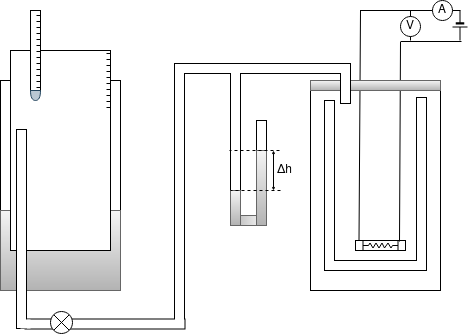
\includegraphics[width=0.5\textwidth]{images/setup-liq-n2.png}
    \caption{\label{fig:setup}Схема на опитна постановка}
    \label{fig:setup}
\end{figure}

\subsection{Извеждане на работна формула}

Топлината, отдадена от нагревателя, може да се определи по формулата на Джаул-Ленц (ур. \ref{eq:joule-lenz}), където $Q$ е отделеното количество топлина, $U$ - пада на напрежението върху нагревателя, $I$ - големината на тока, протичащ през нагревателя, $t$ - времето за нагряване. 

\begin{equation}\label{eq:joule-lenz}
    Q = IUt
\end{equation}
Тъй като дюаровия съд не е напълно топлоизолиран, се налага да отчетем количеството топлина, което води до постоянно изпаряване на течния азот, дори и при изключен нагревател. Това се прави чрез измерване на обемите изпарен азот за едно и също време при включен и изключен нагревател. Тези обеми наричаме съответно $V_1$ и $V_2$. Разликата $V = V_1 - V_2$ дава обема на изпарения азот в резултат само на отделената от нагревателя топлина. От уравнението на Клапейрон-Менделеев (ур. \ref{eq:Mendeleev}) може да се определи масата $M$ на изпарения азот, където $p$ е налягането на газа в газометъра, $R$ - универсалната фазова константа, $T$ - абсолютната температура на газа, $\mu$ - моларната маса на газа. От уравнения \ref{eq:joule-lenz} и \ref{eq:Mendeleev} следва работната ни формула \ref{eq:work-formula}. Налягането $p$ на азота в газометъра определяме по формула \ref{eq:p}, където $\rho$ е плътността на течността в манометъра, $\Delta h$ - разликата в нивата на манометъра, $p_0$ - атмосферното налягане в момента на измерването ([$p_0$] = $Pa$). Обемите $V_1$ и $V_2$ получаваме чрез скалата, закрепена на газометъра, която поради технически причини преобразуваме в друга скала с четири пъти по-голямо деление по формулата $V_{\{1, 2\}} = V_{\{1, 2\}}'\cdot \frac{100}{4}$
\begin{equation}\label{eq:Mendeleev}
    pV = \frac{1}{\mu}MRT
\end{equation}

\begin{equation}\label{eq:work-formula}
    \lambda = \frac{IUtRT}{pV\mu}
\end{equation}

\begin{equation}\label{eq:p}
    p = \rho g \Delta h + p_0
\end{equation}

  
\subsection{Задача: Измерване обемите $V_1$ и $V_2$, налягането $p$, големината на тока $I$ и напрежението $U$ и определяне на стойностите на $\lambda$ за всяка двойка стойности}
Неколкократно измерваме последователно стойностите за $V_1$ и $V_2$, като се отчита и разликата в нивата на диференциалния манометър $\Delta h$ за определяне на налягането $p$. 

Измерванията и резултатите за $\lambda$ записваме в таблица \ref{tbl:results}, като пресмятаме максималната абсолютна грешка с приближението от формула \ref{eq:error}. Използваните константи по време на експеримента са записани в таблица \ref{tbl:params}. Инструменталните грешки определяме като половината от най-малкото деление на записаната в таблица \ref{tbl:params} стойност, съобразявайки се с мерната единица в SI. Инструменталните грешки $\frac{\Delta V}{V} = \frac{\Delta P}{P} = 0.5 mm^3 = 0.5 \cdot 10^{-9} m^3$.

\begin{equation}\label{eq:error}
    \frac{\Delta \lambda}{\lambda} = \frac{\Delta I}{I} + \frac{\Delta U}{U} + \frac{\Delta t}{t} + \frac{\Delta T}{T} + \frac{\Delta p}{p} + \frac{\Delta V}{V} + \frac{\Delta \mu}{\mu}
\end{equation}

\begin{table}[h]
\begin{center}
\begin{tabular}{|l|l|l|l|l|} \hline
    N & V_1', [mm] & V_2', [mm] & \Delta h, [mm] & \lambda, [kJ/kg]\\ \hline
    1 & 34 & 88 & 57 & 203 \pm 5.89 \\ \hline
    2 & 31 & 86 & 56 & 200 \pm 5.79\\ \hline
    3 & 29 & 84 & 57 & 200 \pm 5.79\\ \hline
    4 & 29 & 82 & 58 & 207 \pm 6.00\\ \hline
    5 & 26 & 80 & 59 & 203 \pm 5.89\\ \hline
\end{tabular}
\caption{\label{tbl:results}Измервания и резултати}
\end{center}
\end{table}

\begin{table}[h]
\begin{center}
\begin{tabular}{|l|l|l|} \hline
        $\rho$ на етилов спирт при $T=20 \degree C$& 789.33 $kg/m^3$ \\ \hline
        температура $T$ & 295.15 $K$ \\ \hline
        големина на тока $I$, подадена към нагревателя & 0.72 $A$ \\ \hline 
        пад на напрежение напрежение $U$, & \\
        подаден към нагревателя & 13.8 $V$\\ \hline
        атмосферно налягане $p_0$ & 710.7 $mmHg$ \\ \hline
        земно ускорение $g$ & 9.81 $m/s^2$\\ \hline
        време за нагряване $t$ & 30 $s$\\ \hline
        универсална газова константа $R$ & 8.315 $J/(mol\cdot K)$\\ \hline
        моларна маса $\mu$ на $N_2$ & 28.00134 $g/mol$\\ \hline
\end{tabular}
\caption{\label{tbl:params}Константи по време на експеримента}
\end{center}
\end{table}


\end{document}
